\section{Detecting spoke orders by matrices of full rank}
\label{sec:detector}

Suppose throughout this section that $n=2s+1$, where $s\geq1$, and put
$d=s^2=d_n$.  We construct one linear map on $n\times n$ matrices that
annihilates the additive ambiguity in Lemma~\ref{lem:additive} and every
diagonal matrix, sends
each individual off-diagonal entry to a matrix of rank one, and sends
every matrix recording half the signs of a linear spoke order to an
invertible $d\times d$ matrix.
The last property rests on the following interpolation pattern.

\begin{lemma}[Two-triangle interpolation]
\label{lem:triangular-basis}
For any pairwise distinct real numbers $x_1,\ldots,x_{2s+1}$, set
\begin{equation}
\label{eq:triangular-pattern}
  Q_s=
  \{(p,q):1\leq q<p\leq s+1\}
  \mathbin{\cup}
  \{(p,q):s+1<p<q\leq2s+1\}.
\end{equation}
The values at $(x_p,x_q)$ for $(p,q)\in Q_s$ determine uniquely a
polynomial of degree at most $s-1$ in each variable.
Equivalently, the $s^2$ vectors
\[
  h_{pq}=(x_p^a x_q^b)_{0\leq a,b<s},\qquad (p,q)\in Q_s,
\]
form a basis of $\R^{s^2}$, with the coordinates taken in any fixed order.
\end{lemma}

Figure~\ref{fig:triangular-grid} shows the pattern $Q_s$ and the two
eliminations in the inductive proof.
\begin{figure}[hb]
\centering
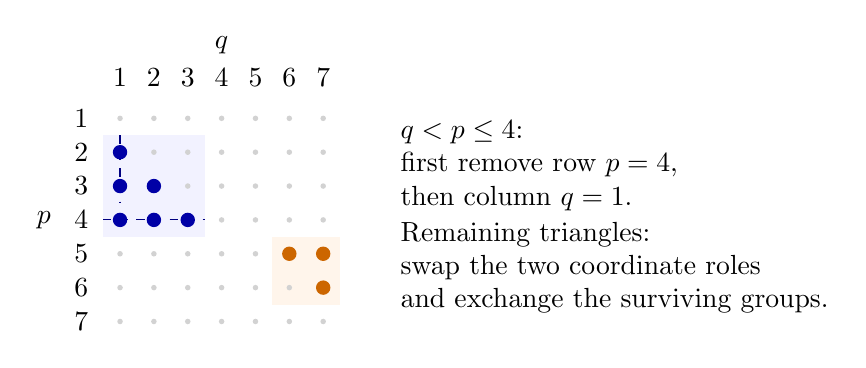
\begin{tikzpicture}[x=.43cm,y=-.43cm]
  \fill[blue!5] (.5,1.5) rectangle (3.5,4.5);
  \fill[orange!8] (5.5,4.5) rectangle (7.5,6.5);
  \draw[blue!50!black,dashed] (.5,4)--(3.5,4);
  \draw[blue!50!black,dashed] (1,1.5)--(1,3.5);
  \foreach \p in {1,...,7}{
    \node[left] at (.35,\p) {$\p$};
    \node[above] at (\p,.35) {$\p$};
    \foreach \q in {1,...,7}{
      \fill[gray!35] (\q,\p) circle (1.0pt);
    }
  }
  \foreach \p/\q in {2/1,3/1,3/2,4/1,4/2,4/3}
    \fill[blue!65!black] (\q,\p) circle (2.6pt);
  \foreach \p/\q in {5/6,5/7,6/7}
    \fill[orange!80!black] (\q,\p) circle (2.6pt);
  \node at (-1.25,4) {$p$};
  \node at (4,-1.15) {$q$};
  \node[anchor=west,align=left] at (9,2.4)
    {$q<p\le4$:\\first remove row $p=4$,\\then column $q=1$.};
  \node[anchor=west,align=left] at (9,5.4)
    {Remaining triangles:\\swap the two coordinate roles\\and exchange the surviving groups.};
\end{tikzpicture}
\caption{The evaluation pattern $Q_s$ for $s=3$, with $n=7$ and $s^2=9$
selected pairs. Removing row $p=s+1$ and then column $q=1$
leaves the pattern for $s-1$ after swapping coordinates and
relabeling the two groups. The gray points are unselected pairs.}
\label{fig:triangular-grid}
\end{figure}


\begin{proof}
The polynomial space has dimension $s^2$, and
\[
  |Q_s|=\frac{s(s+1)}2+\frac{s(s-1)}2=s^2.
\]
It therefore suffices to show that a polynomial $P(u,v)$ of degree at
most $s-1$ in each variable, vanishing at all these points, is zero.
We prove this by induction on $s$.  For $s=1$, $P$ is constant and
vanishes at the single point indexed by $(2,1)$.

Let $s>1$.  The first triangle contains the $s$ points
$(x_{s+1},x_q)$ for $1\leq q\leq s$.  The polynomial
$P(x_{s+1},v)$ has degree at most $s-1$ and $s$ distinct roots, so it
vanishes identically.  Division in the variable $u$ gives
\[
  P(u,v)=(u-x_{s+1})P_1(u,v),
  \qquad \deg_u P_1\leq s-2,\quad\deg_v P_1\leq s-1.
\]
For $p=2,\ldots,s$, the remaining points $(x_p,x_1)$ give
$P_1(x_p,x_1)=0$, since $x_p\ne x_{s+1}$.  Thus
$P_1(u,x_1)$, of degree at most $s-2$, has $s-1$ distinct roots and
vanishes identically.  Factoring in the second variable, we obtain
\begin{equation}
\label{eq:triangle-factorization}
  P(u,v)=(u-x_{s+1})(v-x_1)R(u,v),
  \qquad \deg_u R,\deg_v R\leq s-2.
\end{equation}
At every point in the two remaining triangles the displayed factors
are nonzero.  Hence
\[
  R(x_p,x_q)=0
  \quad\text{if }2\leq q<p\leq s
  \quad\text{or if }s+2\leq p<q\leq2s+1.
\]
Define a tuple of $2s-1$ distinct nodes and a polynomial by
\[
  (y_1,\ldots,y_{2s-1})
   =(x_{s+2},\ldots,x_{2s+1},x_2,\ldots,x_s),
  \qquad S(u,v)=R(v,u).
\]
The lower triangle $q<p\leq s$ for the $y$-tuple becomes the remaining
upper triangle for the $x$-tuple after the coordinate swap.  The upper
triangle $s<p<q\leq2s-1$ becomes the remaining lower triangle.
Consequently $S$ vanishes at every point of the pattern $Q_{s-1}$ for
the $y$-tuple.  The induction hypothesis gives $S=0$, hence $R=0$ and
$P=0$.  This proves injectivity of the square evaluation map and thus
both assertions.
\end{proof}

\begin{lemma}[Rank detector]
\label{lem:detector}
Fix any pairwise distinct real numbers $x_1,\ldots,x_n$, where
$n=2s+1$ and $d=s^2$.  There is a linear map
$\Phi:\R^{n\times n}\longrightarrow\R^{d\times d}$ with the following
properties.
\begin{enumerate}[label=\textup{(\roman*)}]
\item $\Phi$ annihilates every additive matrix
$H(p,q)=r_p+c_q$ and every diagonal matrix.
\item For the coordinate matrix $E_{pq}$, the matrix $\Phi(E_{pq})$
has rank one if $p\ne q$, and is zero if $p=q$.
\item For every strict linear order $\prec$ on $\{1,\ldots,n\}$, the
matrix $\Phi(S_\prec)$ is invertible, where
\[
  S_\prec(p,q)=
  \begin{cases}
    \tfrac12,&p\prec q,\\
    -\tfrac12,&q\prec p,\\
    0,&p=q.
  \end{cases}
\]
\end{enumerate}
The same map has these properties for all orders simultaneously.
\end{lemma}

\begin{proof}
Set
\begin{equation}
\label{eq:detector-definition}
\begin{gathered}
  F(t)=\prod_{p=1}^{n}(t-x_p),\qquad
  h_{pq}=(x_p^a x_q^b)_{0\leq a,b<s},\\
  B_{pq}=\frac{x_p-x_q}{F'(x_p)F'(x_q)}
              h_{pq}h_{pq}^{\mathsf T},\qquad
  \Phi(H)=\sum_{p,q=1}^{n}H(p,q)B_{pq}.
\end{gathered}
\end{equation}
The factors $1/F'(x_p)$ are the classical barycentric weights for Lagrange
interpolation~\cite[Section~3, equation~(3.2)]{BerrutTrefethen2004}.
All denominators are nonzero because the nodes are distinct.
The constant coordinate of $h_{pq}$ is $1$, so $B_{pq}$ has rank one
when $p\ne q$, while $B_{pp}=0$.  This proves \textup{(ii)} and the
annihilation of diagonal matrices.  Rank subadditivity also gives
\begin{equation}
\label{eq:detector-support-bound}
  \rank\Phi(H)\leq
  \bigl|\{(p,q):p\ne q,\ H(p,q)\ne0\}\bigr|.
\end{equation}

For the additive matrices, we use the elementary identity
\begin{equation}
\label{eq:lagrange-vanishing}
  \sum_{p=1}^{n}\frac{A(x_p)}{F'(x_p)}=0
  \qquad\text{if }\deg A\leq n-2.
\end{equation}
Indeed, the polynomials
$F(t)/((t-x_p)F'(x_p))$ have degree $n-1$ and take the coordinate
values $1$ at $x_p$ and $0$ at every other node.  Subtracting their
linear combination with coefficients $A(x_p)$ from $A$ gives a
polynomial of degree at most $n-1$ with $n$ distinct roots, so
\[
  A(t)=\sum_{p=1}^{n}
        A(x_p)\frac{F(t)}{(t-x_p)F'(x_p)}.
\]
Comparison of the coefficients of $t^{n-1}$ proves
\eqref{eq:lagrange-vanishing}.

The entry of $B_{pq}$ indexed by $(a,b)$ and $(a',b')$ is
\[
  \frac{(x_p-x_q)x_p^{a+a'}x_q^{b+b'}}
       {F'(x_p)F'(x_q)}.
\]
Its numerator has degree at most $2s-1=n-2$ in either variable
separately.  Applying \eqref{eq:lagrange-vanishing} with the other
variable fixed proves
\[
  \sum_{q=1}^{n}B_{pq}=0\quad\text{for every }p,
  \qquad
  \sum_{p=1}^{n}B_{pq}=0\quad\text{for every }q.
\]
It follows that $\Phi((r_p+c_q)_{p,q})=0$, completing \textup{(i)}.

It remains to prove \textup{(iii)}.  First take the natural order and
write $S=S_\prec$.  Let $H(p,q)=\mathbf{1}_{q<p}$ and let $\mathbf1$
denote the all-ones column vector.  Then
\[
  S=\tfrac12\mathbf1\mathbf1^{\mathsf T}-H-\tfrac12I_n,
  \qquad \Phi(S)=-\Phi(H).
\]
Subtract $1$ from each row of $H$ indexed by $p>s+1$, obtaining
$H'$.  The difference $H-H'$ is additive, so $\Phi(H')=\Phi(H)$.
Apart from diagonal entries, which $\Phi$ annihilates, the support
of $H'$ is exactly $Q_s$: its value is $+1$ on the first triangle
of \eqref{eq:triangular-pattern} and $-1$ on the second.

List the pairs in $Q_s$ in any order, and let $A_Q$ be the square
matrix with columns $h_{pq}$ in that order.  By
Lemma~\ref{lem:triangular-basis}, $A_Q$ is invertible.  Equation
\eqref{eq:detector-definition} now gives
\begin{equation}
\label{eq:detector-factorization}
  \Phi(S)=-A_Q D_Q A_Q^{\mathsf T},\qquad
  D_Q=\diag\left(
       H'(p,q)\frac{x_p-x_q}{F'(x_p)F'(x_q)}
       \right)_{(p,q)\in Q_s}.
\end{equation}
Every diagonal entry of $D_Q$ is nonzero, so $\Phi(S)$ is invertible.

Finally let $\pi(1)\prec\cdots\prec\pi(n)$ be an arbitrary order.
Relabel the indices and use the tuple
$(x_{\pi(1)},\ldots,x_{\pi(n)})$ in the argument just given.
The relabeled evaluation vector at $(r,q)$ is
$h_{\pi(r),\pi(q)}$, so this only reindexes the sum defining
$\Phi(S_\prec)$; the polynomial $F$ and the fixed map $\Phi$ are
unchanged.  The relabeled nodes are
distinct, so Lemma~\ref{lem:triangular-basis} applies again.
Thus every order has invertible image under the original map.
\end{proof}
